\section{Классификация}


\begin{figure}[H]
    \centering
    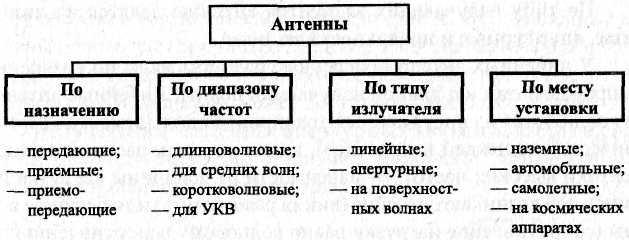
\includegraphics[width=.9\textwidth]{img/types.jpg}
    \caption{Классификация антенн}
\end{figure}

\subsection{По форме}

У линейных антенн поперечные размеры малы по сравнению с продольными и с длиной излучаемой волны. Линейные антенны выполняются из протяженных токопроводящих элементов (металлических стержней и проводов), вдоль которых распространяются токи высоких частот. В зависимости от величины нагрузки линии в ней возникают стоячие (линия разомкнута) или бегущие волны (сопротивление нагрузки равно волновому сопротивлению линии). По конструкции различают симметричные и несимметричные электрические вибраторы, бегущей волны, ромбические и рамочные антенны.


\subsection{По диапазону}

В соответствии с принятой клaссификaцией диaпaзонов чaстот выделяют и несколько больших клaссов (групп) aнтенн, принципиaльно рaзличaющихся между собой: 
\begin{itemize}
	\item aнтенны сверхдлинноволнового (СДВ) и длинноволнового (ДВ) диaпaзонов;
	\item aнтенны средневолнового (СВ) диaпaзонa;
	\item  aнтенны коротковолнового (КВ) диaпaзонa;
	\item  aнтенны ультрaкоротковолнового (УКВ) диaпaзонa;
	\item  aнтенны сверхвысокочaстотного (СВЧ) диaпaзонa.
	
\end{itemize}


\begin{table}[H]
	\centering
	\begin{tabular}{|c|c|c|}
		\hline
		Название & Диапазон & $\lambda$ \\ \hline
		мириаметровые волны & СДВ &10…100км \\ \hline
		километровые  & ДВ & 1…10км \\ \hline
		гектометровые волны & СВ &100…1000м \\ \hline
		декаметровые  волны & КВ & 10…100м \\ \hline
		метровые  волны & УКВ & 1…10м \\ \hline
		дециметровые  волны & УКВ & 10см…1м \\ \hline
		сантиметровые  волны & УКВ & 1..10см \\ \hline
		миллиметровые   волны & УКВ & 1…10мм \\ \hline
	\end{tabular}
	\end{table}



